\documentclass[letterpaper,11pt]{article}

\usepackage[utf8]{inputenc}
\usepackage[spanish,mexico]{babel}
\usepackage{graphicx}
\usepackage{amsmath}
\usepackage{amsthm}
\usepackage{svg}
\usepackage{amsfonts}
\usepackage{subcaption}
\usepackage[hmargin=1in, vmargin=1in]{geometry}
\usepackage{fancyhdr}
\pagestyle{fancy}
\usepackage{tasks}
\lhead{\ExiCarrera}
\chead{\ExiMateria}
\rhead{\ExiParcial}
\cfoot{\ExiEscuela}
\renewcommand{\headrulewidth}{0.4pt}
\renewcommand{\footrulewidth}{0.4pt}

\providecommand{\abs}[1]{\lvert#1\rvert}
\providecommand{\norm}[1]{\lVert#1\rVert}

\newcommand{\informacion}[1]{
\begin{center}
\fbox{\fbox{\parbox{\textwidth}{{\footnotesize#1}}}}
\end{center}
\vspace{5mm}}
\newcommand{\datos}{\makebox[0.7\textwidth]{Nombre:~\hrulefill} Fecha:~\hrulefill}
\newcommand{\pregunta}[2]{\item{#2}~{(#1 puntos)}\\ \vspace{5mm}						       
			{\bf Solución}}														  
\newcommand{\ExiCarrera}{Matemáticas para las Ciencias II.}											 
\newcommand{\ExiMateria}{\textbf{Proyecto II}}														
\newcommand{\ExiParcial}{Entrega: Viernes 20 de Marzo}														  
\newcommand{\ExiEscuela}{\textbf{Facultad de Ciencias, UNAM}}	                		    
\begin{document}
\setlength{\unitlength}{1cm}
\thispagestyle{empty}
\begin{picture}(18,4)
\put(-0.5,1.2){
\includegraphics[scale=.25]{unam1.png}}
\put(13.5,1){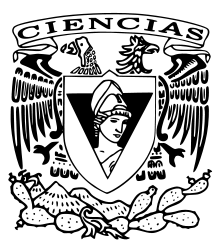
\includegraphics[scale=.35]{fciencias1.png}}
\end{picture}

\begin{center}
\vspace{-134pt}
\textbf{\large Matemáticas para las Ciencias II}\\[0.2cm]
\textbf{ Semestre 2020-1}\\[0.2cm]
Prof. Pedro Porras Flores\\[0.2cm]
Ayud. Irving Hérnandez Rosas \\ [0.2cm]
Kevin Ariel Merino Peña\\
\textbf{Proyecto II}
\end{center}
\vspace{-10pt}
\rule{17cm}{0.3mm}
\begin{flushright}
\vspace{-3pt}
\end{flushright}

\noindent Realice los siguientes ejercicios, escribiendo el procedimiento claramente. Y recuerden que estos proyectos se entregan de manera individual en la plataforma de google classroom. 


\begin{enumerate}

% -----------------------------------------------------
% Problema uno
% -----------------------------------------------------

\item  Sea $f:\mathbb{R}^2 \longrightarrow \mathbb{R}$, tal que $f(x,y) = 9x^2 + y^2$, realice los siguientes bosquejos: 


a) Las curvas de nivel para $f$ para $c \in \{0, 1, 9\}$.
\begin{figure}[h!]
	\centering
	\begin{subfigure}{0.3\textwidth}
		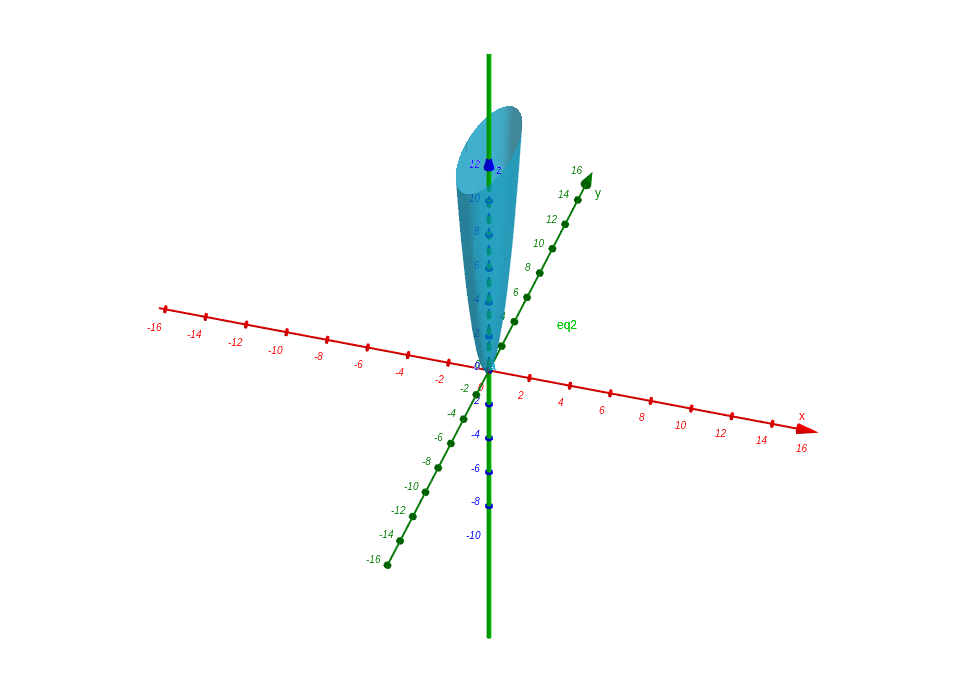
\includegraphics[width=\linewidth]{img/1a1}
		\caption{Con $ c = 0 $}
	\end{subfigure}
	\begin{subfigure}{0.3\textwidth}
		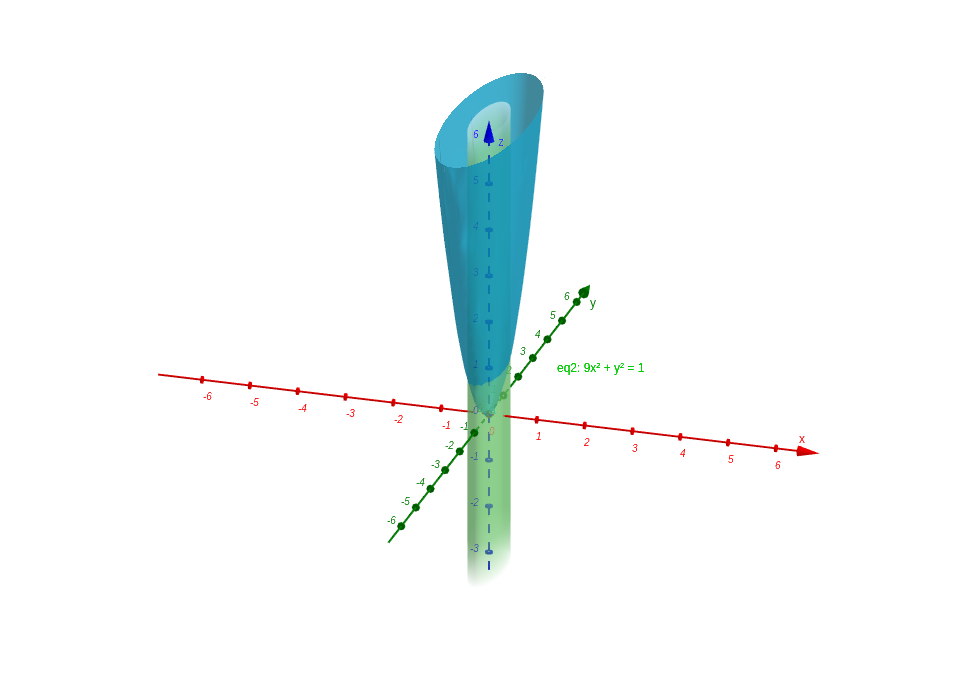
\includegraphics[width=\linewidth]{img/1a2}
		\caption{Para $ c = 1 $}
	\end{subfigure}
	\begin{subfigure}{0.3\textwidth}
		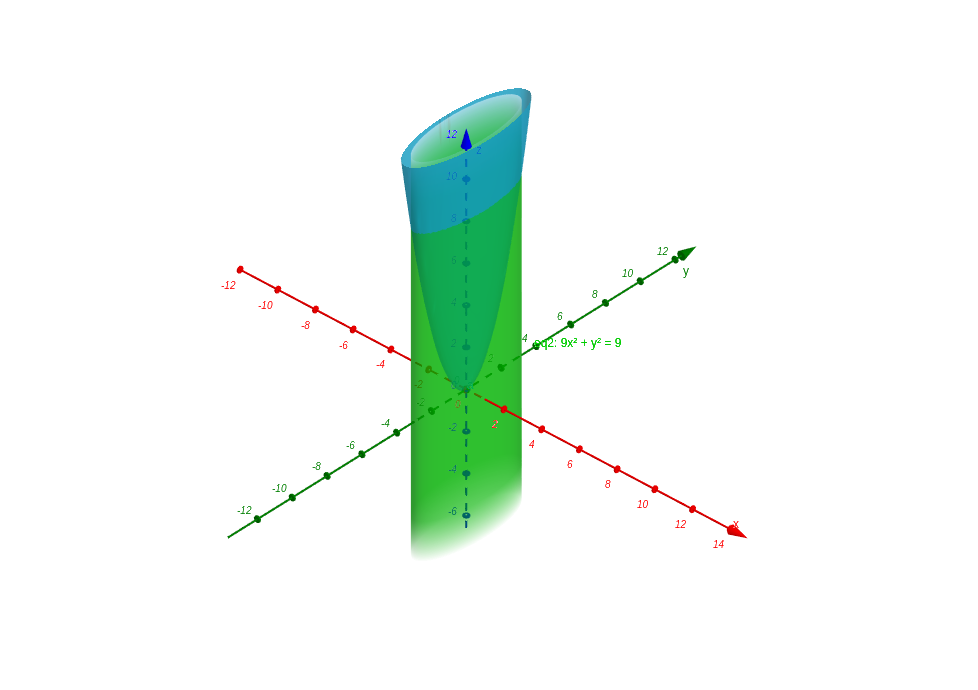
\includegraphics[width=\linewidth]{img/1a3}
		\caption{Para $ c = 9 $}
	\end{subfigure}
	\caption{Curvas de nivel }
\end{figure}

b) Secciones de gráfica de $f$ con los planos $x = -1$, $x = 0$ y $x = 1$.\\
\begin{figure}[h!]
	\centering
	\begin{subfigure}{0.3\textwidth}
		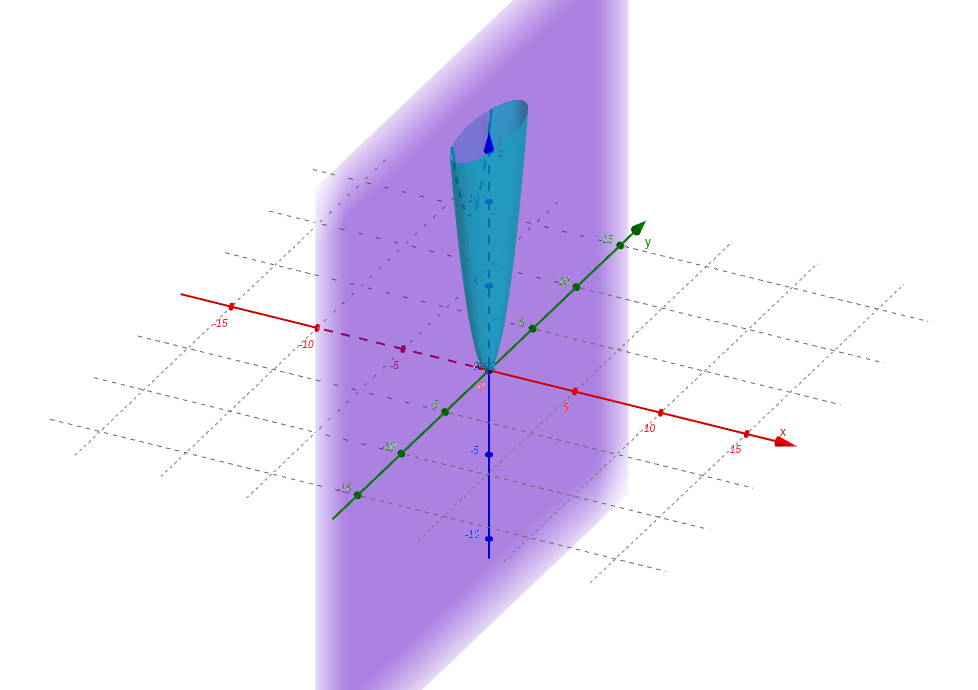
\includegraphics[width=\linewidth]{img/1b1}
		\caption{Con $ x = -1 $}
	\end{subfigure}
	\begin{subfigure}{0.3\textwidth}
		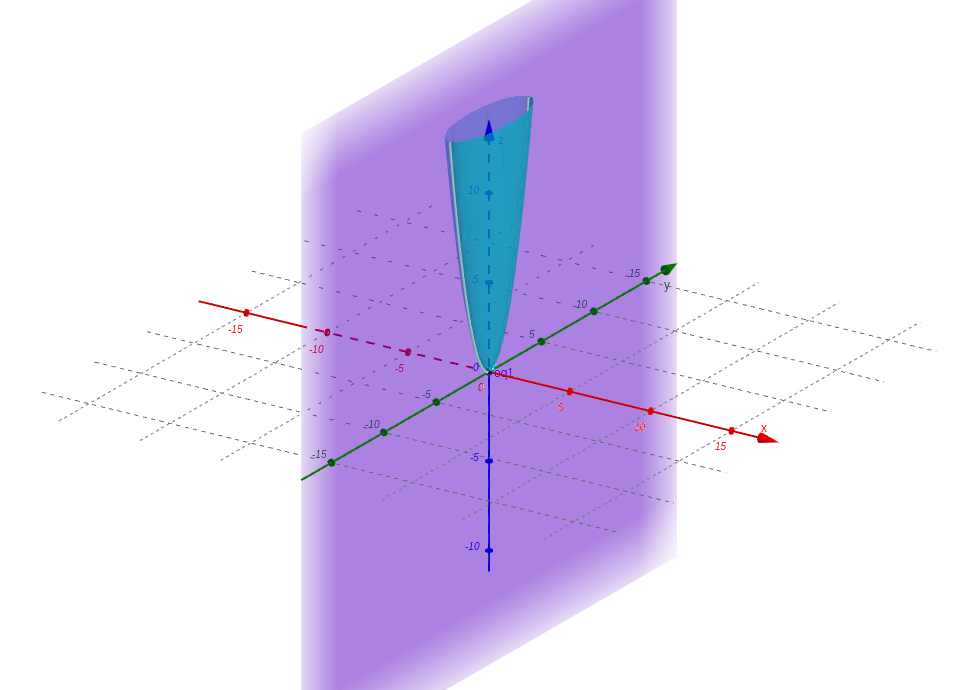
\includegraphics[width=\linewidth]{img/1b2}
		\caption{Para $ x = 0 $}
	\end{subfigure}
	\begin{subfigure}{0.3\textwidth}
		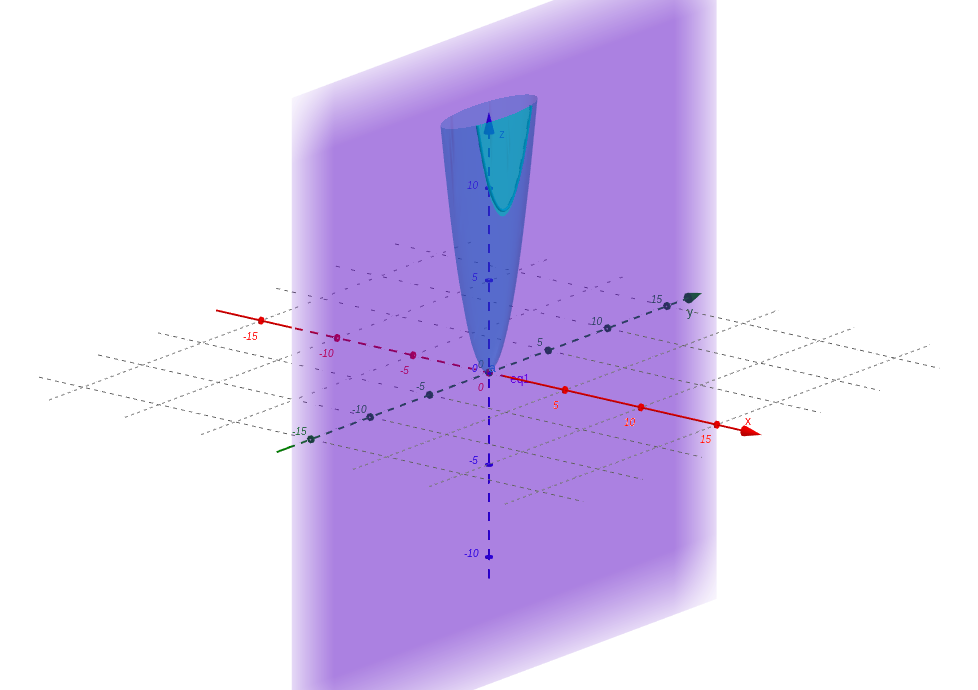
\includegraphics[width=\linewidth]{img/1b3}
		\caption{Para $ x = 1 $}
	\end{subfigure}
	\caption{Secciones de la gráfica }
\end{figure}\\
c) Secciones de gráfica de $f$ con los planos $y = -1$, $y = 0$ y $y = 1$.\\
\begin{figure}[h!]
	\centering
	\begin{subfigure}{0.3\textwidth}
		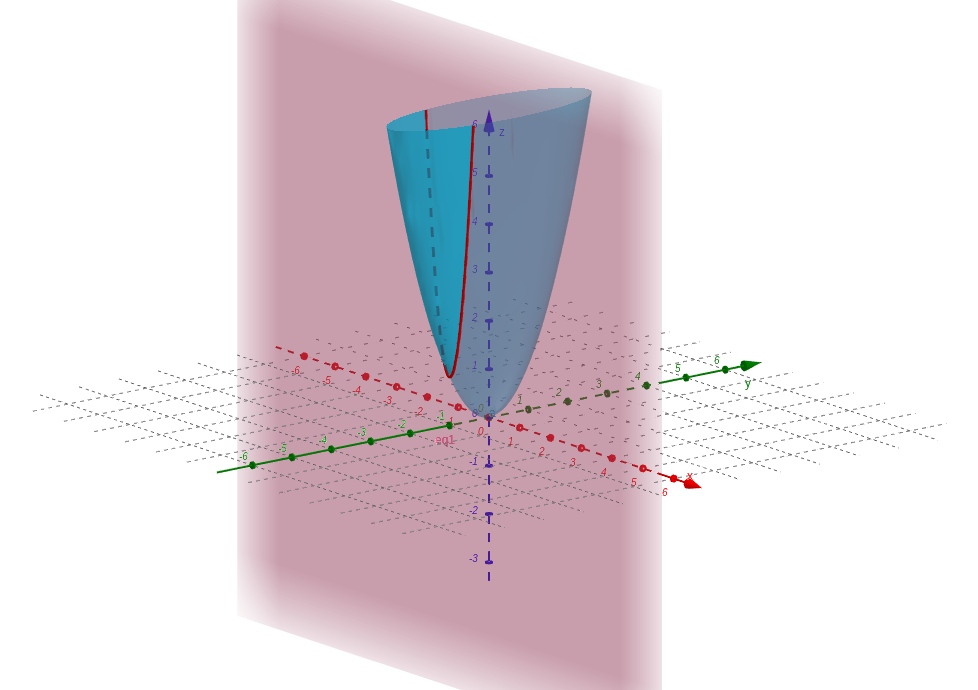
\includegraphics[width=\linewidth]{img/1c1}
		\caption{Con $ y = -1 $}
	\end{subfigure}
	\begin{subfigure}{0.3\textwidth}
		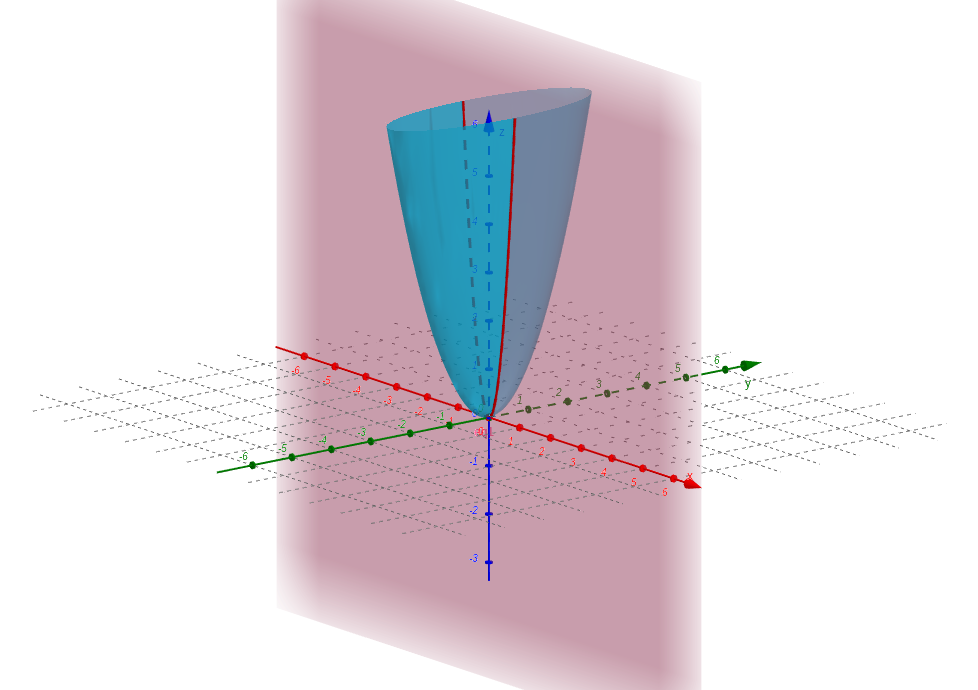
\includegraphics[width=\linewidth]{img/1c2}
		\caption{Para $ y = 0 $}
	\end{subfigure}
	\begin{subfigure}{0.3\textwidth}
		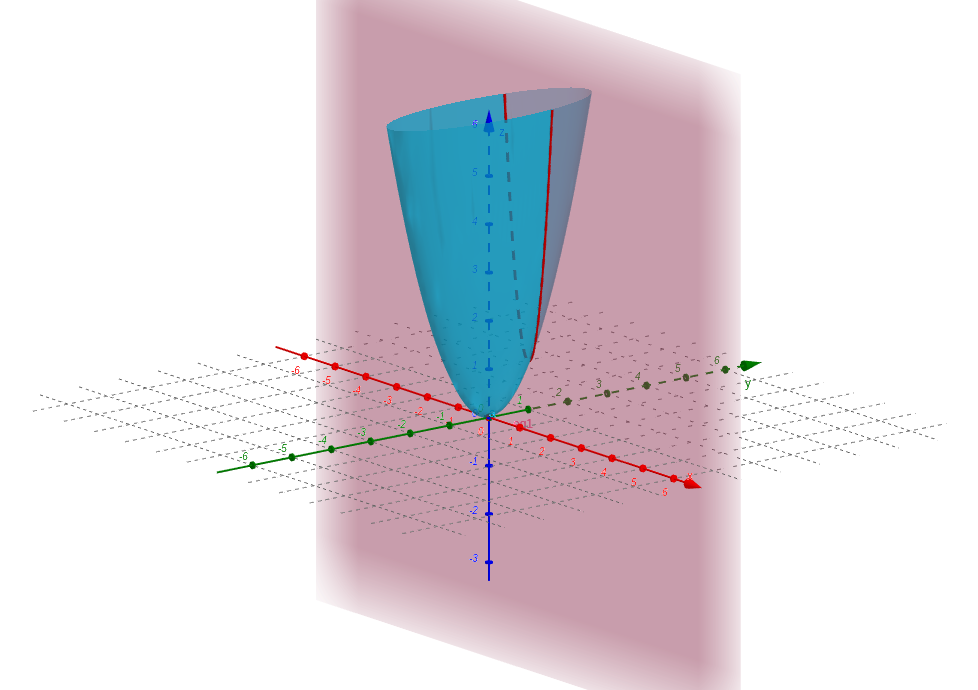
\includegraphics[width=\linewidth]{img/1c3}
		\caption{Para $ y = 1 $}
	\end{subfigure}
	\caption{Secciones de la gráfica }
\end{figure}\\
\newpage
d) La grafica de $f$\\
\begin{figure}[h!]
	\centering
	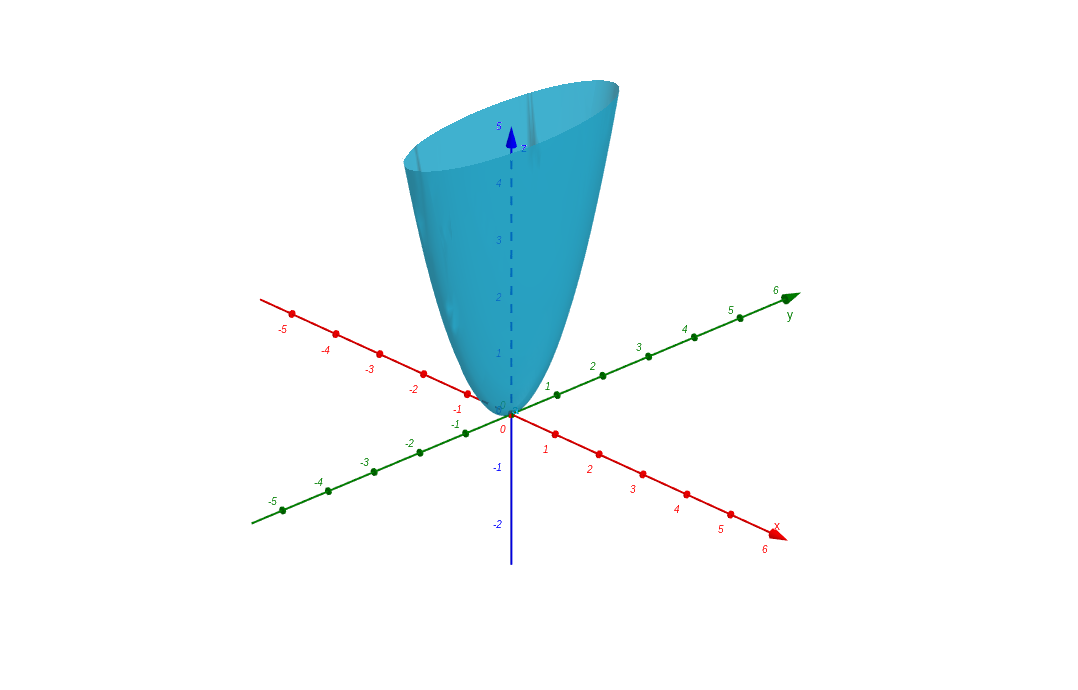
\includegraphics[width=15cm]{img/1d}
	\caption{La gráfica de $ f $}
\end{figure}
\newpage
\item Describa la siguiente función $f:\mathbb{R}^3 \longrightarrow \mathbb{R}$, tal que $f(x,y,z) = 4x^2-3y^2+2z^2$, usando superficies de nivel y a su vez describa éstas superficies con curvas de nivel y secciones. Incluya algunas gráficas.

\begin{figure}[h]
	\centering
	\begin{subfigure}{.7\textwidth}
		\centering
		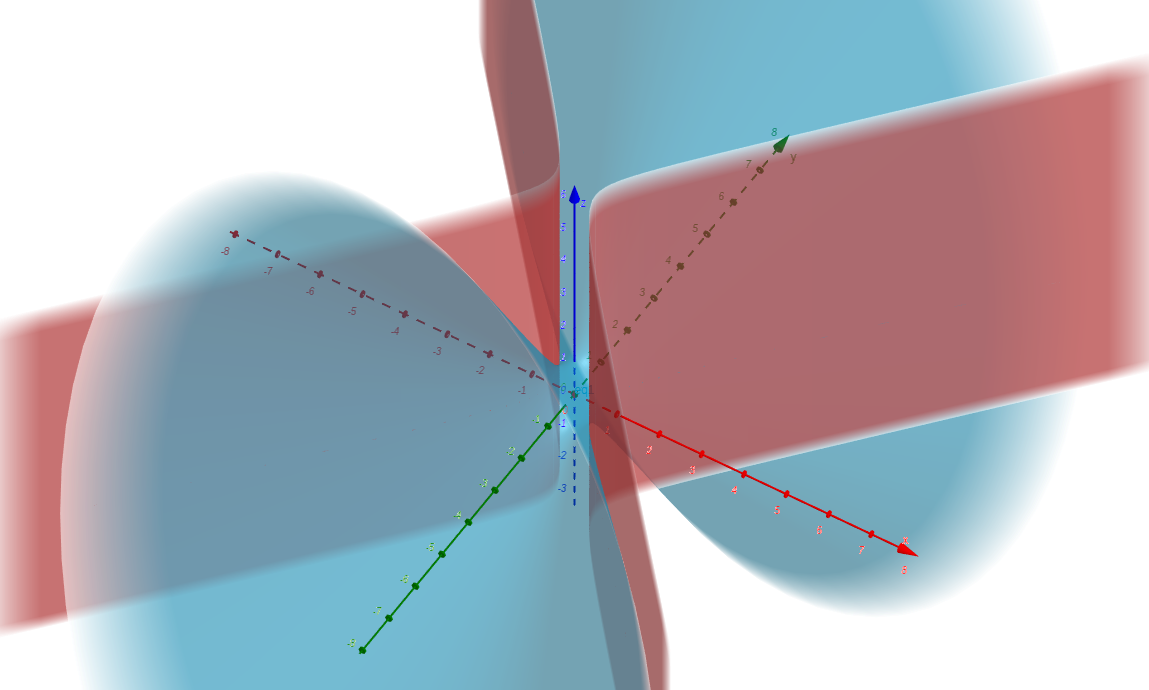
\includegraphics[width=8cm]{img/2a1}
		\caption{Superficie de nivel con $z = 0$.}
		\label{F1_1}
	\end{subfigure}
	\begin{subfigure}{.4\textwidth}
		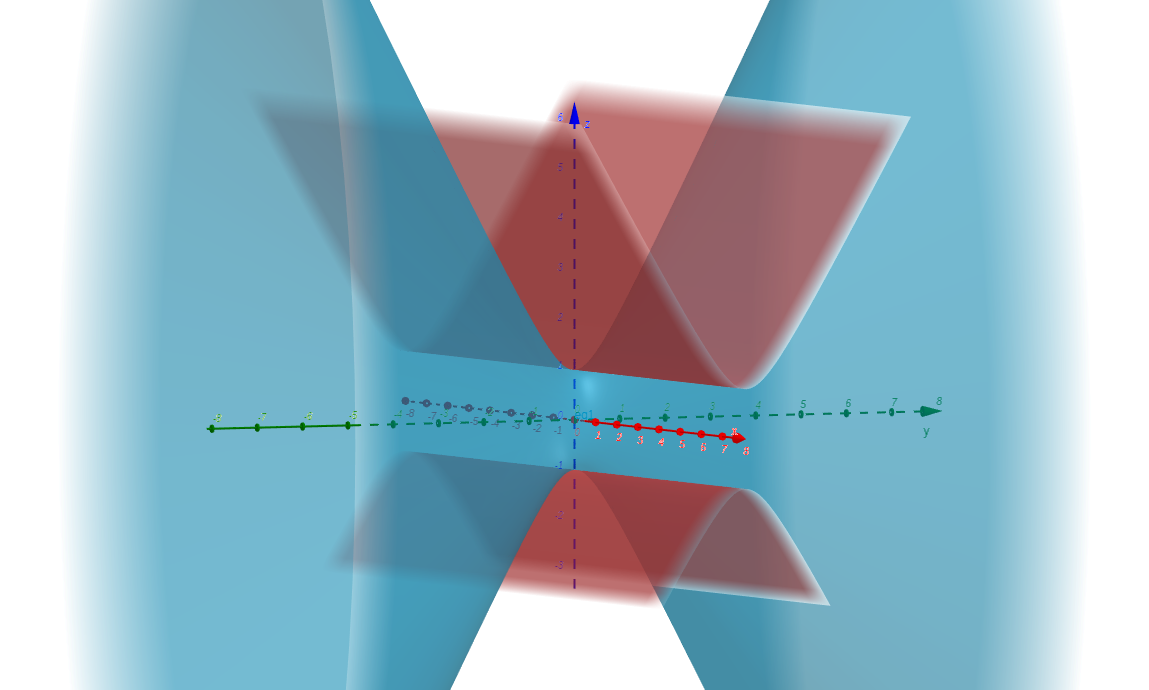
\includegraphics[width=\linewidth]{img/2a2}
		\caption{Superficie de nivel con $x = 0$.}
		\label{F1_2}
	\end{subfigure}
	\begin{subfigure}{.4\textwidth}
		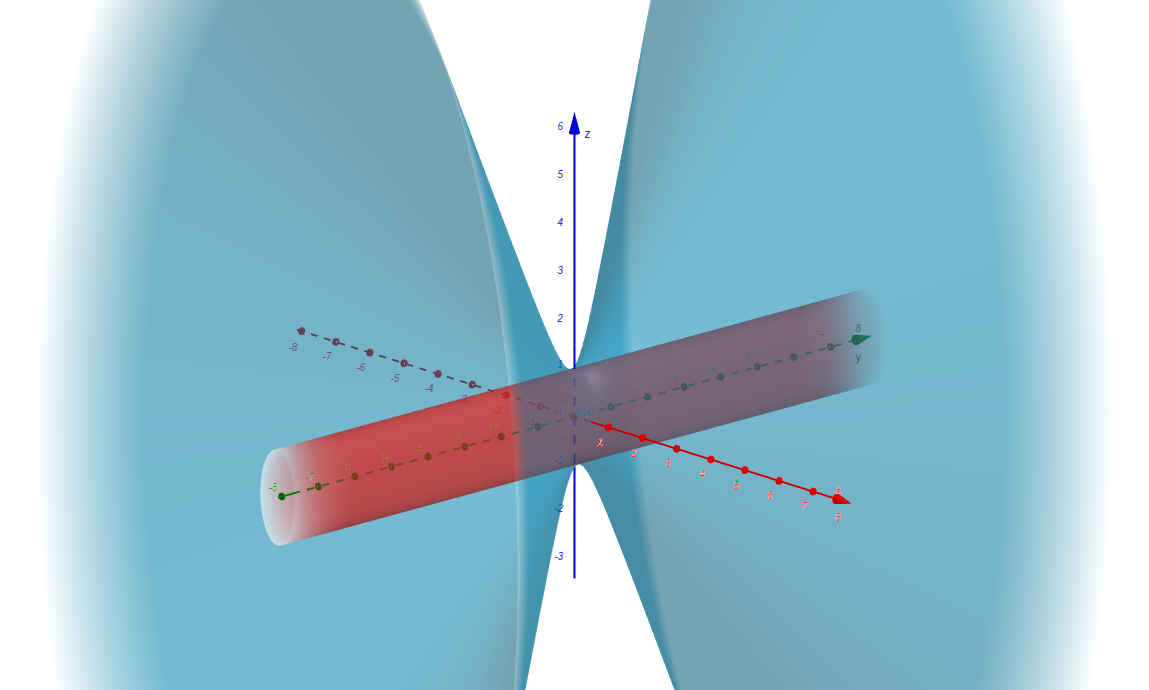
\includegraphics[width=\linewidth]{img/2a3}
		\caption{Superficie de nivel con $x = 0$.}
		\label{F1_3}
	\end{subfigure}
\begin{subfigure}{0.5\textwidth}
	\centering
	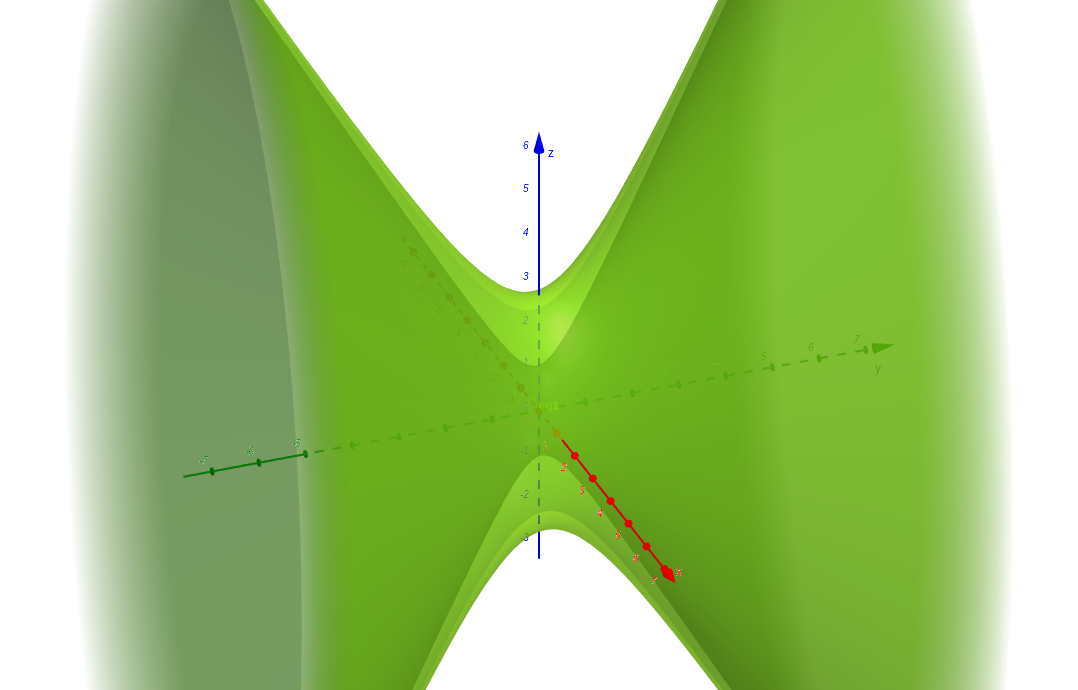
\includegraphics[width=\linewidth]{img/2b1}
	\caption{Superficies de nivel Superpuestas}
\end{subfigure}
	\caption{Superficies de nivel}
	\label{F1}
\end{figure}
\begin{figure}[h!]
	\centering
	\begin{subfigure}{.7\textwidth}
		\centering
		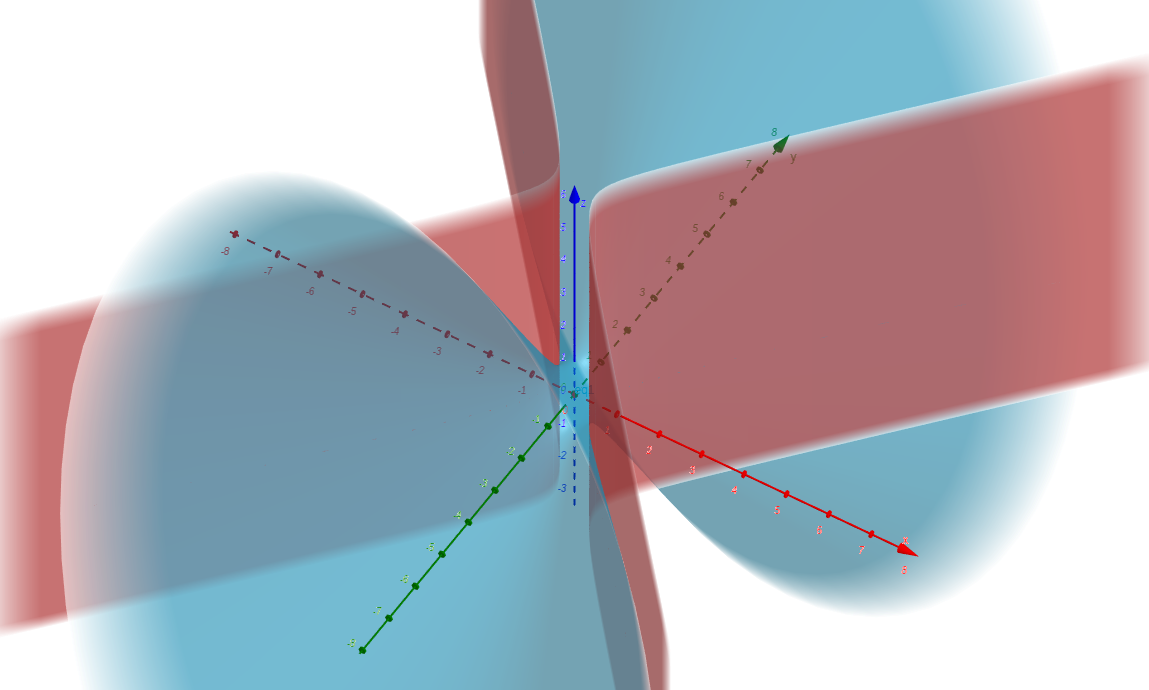
\includegraphics[width=9cm]{img/2a1}
		\caption{Tomaremos la superficie roja }
		\label{F1_1}
	\end{subfigure}
	\begin{subfigure}{0.3\textwidth}
		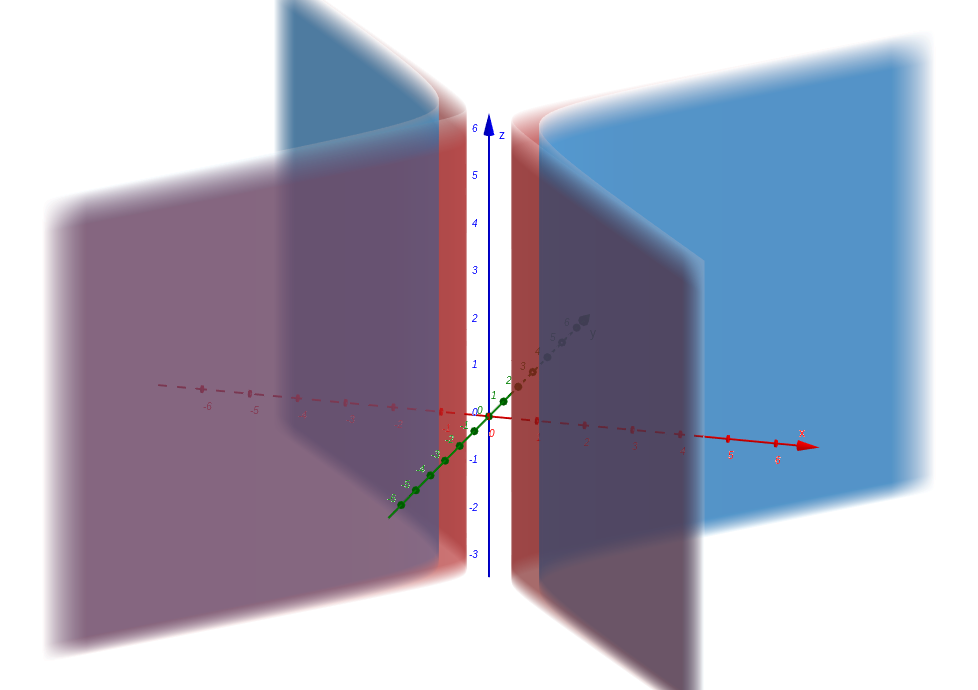
\includegraphics[width=\linewidth]{img/2c1}
		\caption{Con $ c = 5 $}
	\end{subfigure}
	\begin{subfigure}{0.3\textwidth}
		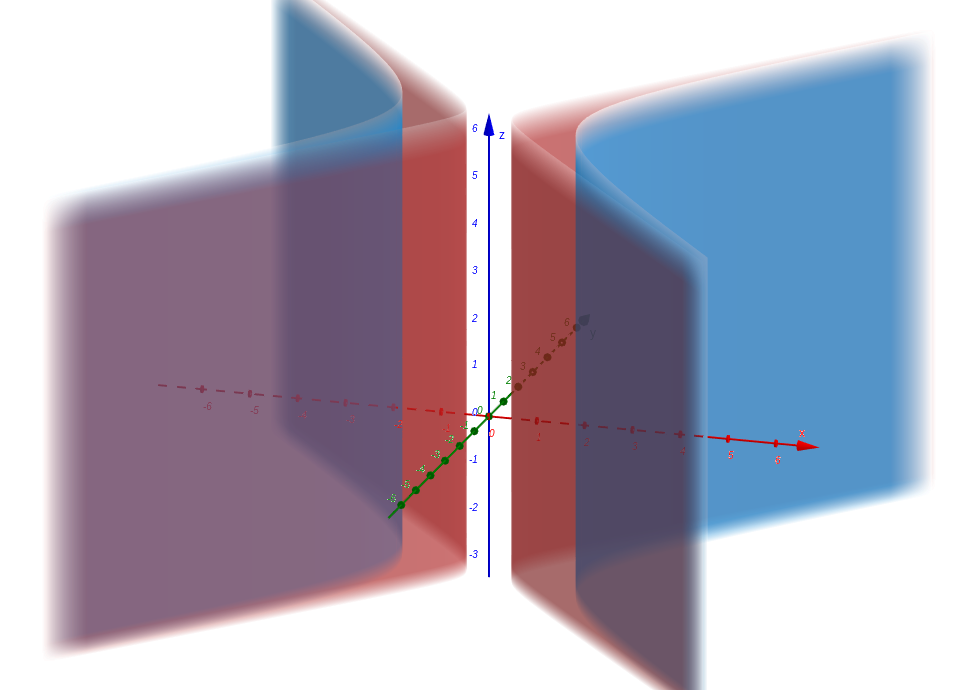
\includegraphics[width=\linewidth]{img/2c2}
		\caption{Para $ c = 20 $}
	\end{subfigure}
	\begin{subfigure}{0.3\textwidth}
		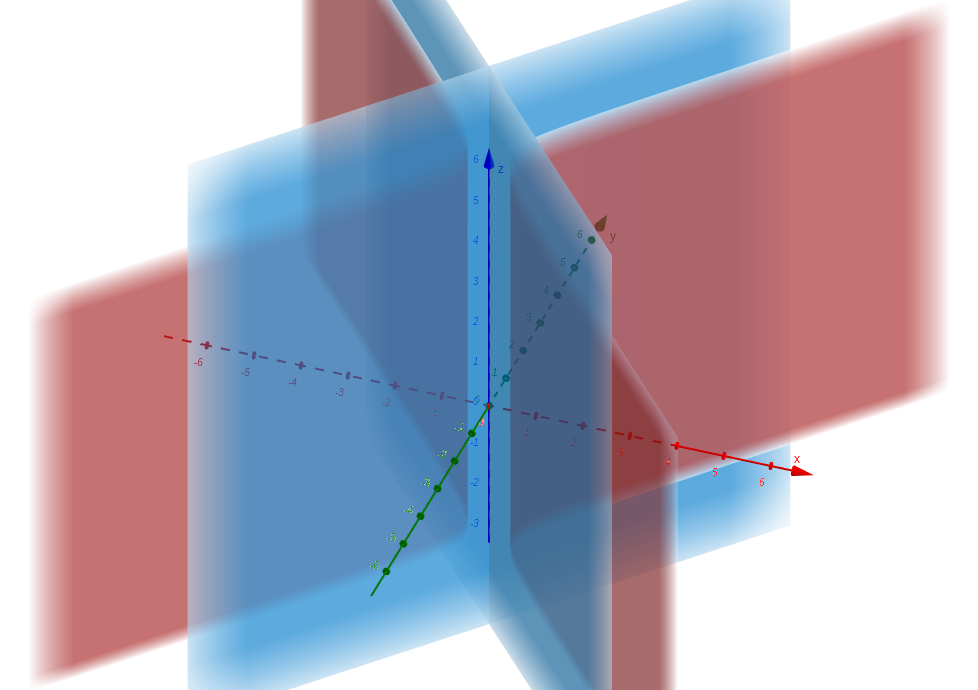
\includegraphics[width=\linewidth]{img/2c3}
		\caption{Para $ c = 0 $}
	\end{subfigure}
	\caption{Secciones de la gráfica }
\end{figure}
\begin{figure}[h!]
	\centering
	\begin{subfigure}{.7\textwidth}
		\centering
		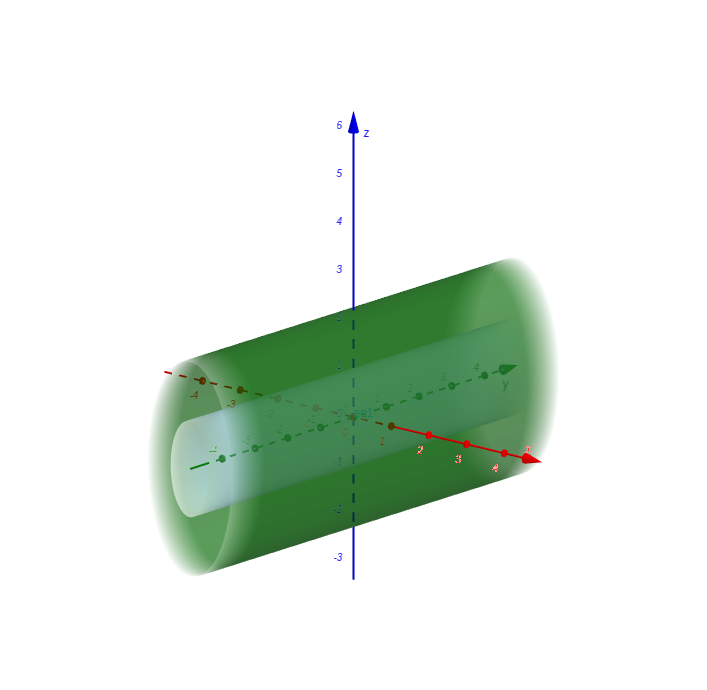
\includegraphics[width=9cm]{img/2d1}
		\caption{Tomaremos la superficie verde }
		\label{F1_1}
	\end{subfigure}
	\begin{subfigure}{0.3\textwidth}
		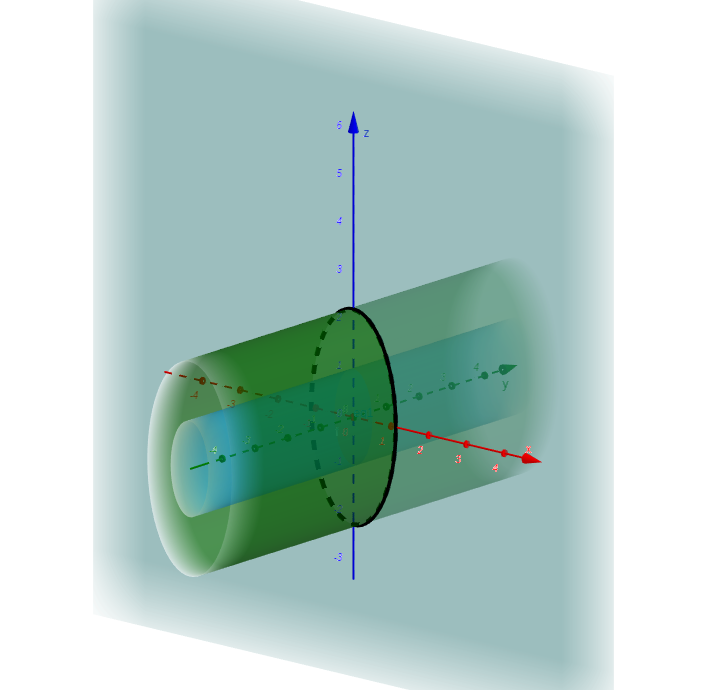
\includegraphics[width=\linewidth]{img/2d1_1}
		\caption{Con $ y = 5 $}
	\end{subfigure}
	\begin{subfigure}{0.3\textwidth}
		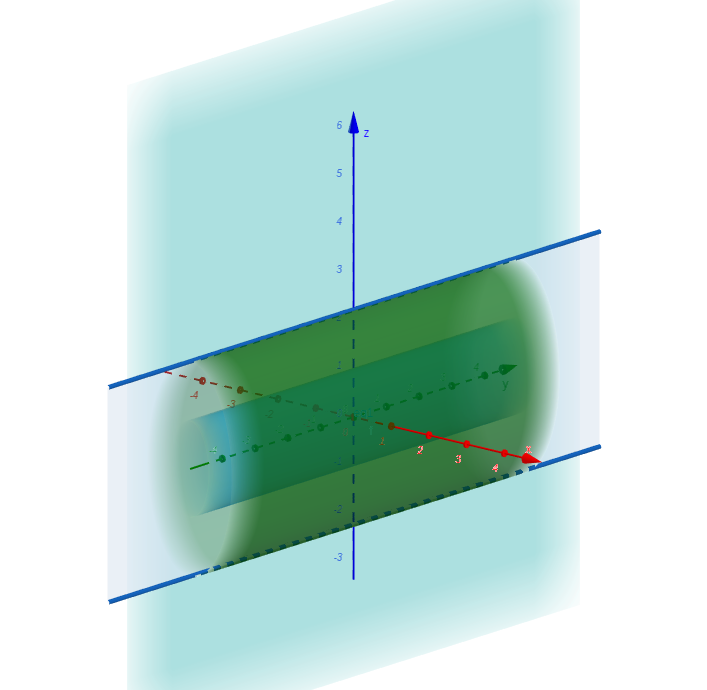
\includegraphics[width=\linewidth]{img/2d1_2}
		\caption{Para $ x = 20 $}
	\end{subfigure}
	\begin{subfigure}{0.3\textwidth}
		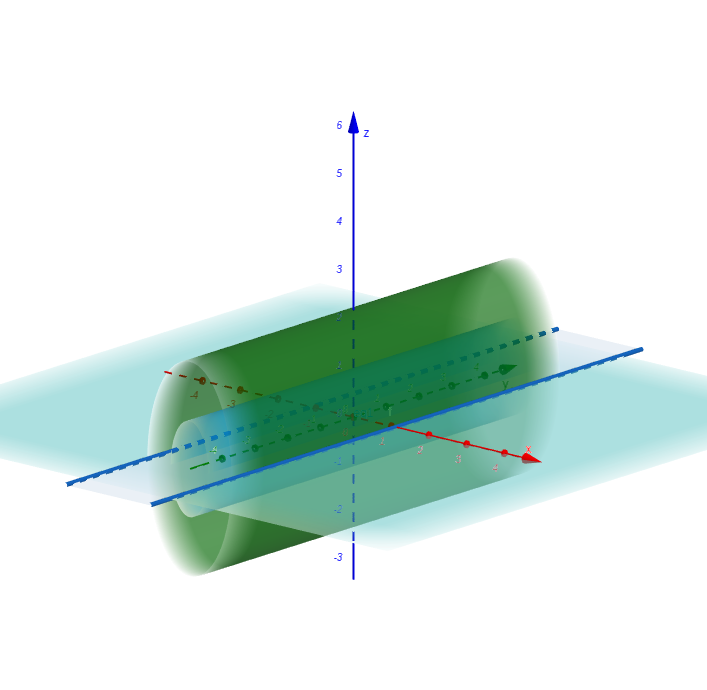
\includegraphics[width=\linewidth]{img/2d1_3}
		\caption{Para $ z = 0 $}
	\end{subfigure}
	\caption{Secciones de la gráfica }
\end{figure}
\begin{figure}[h!]
	\centering
	\begin{subfigure}{.7\textwidth}
		\centering
		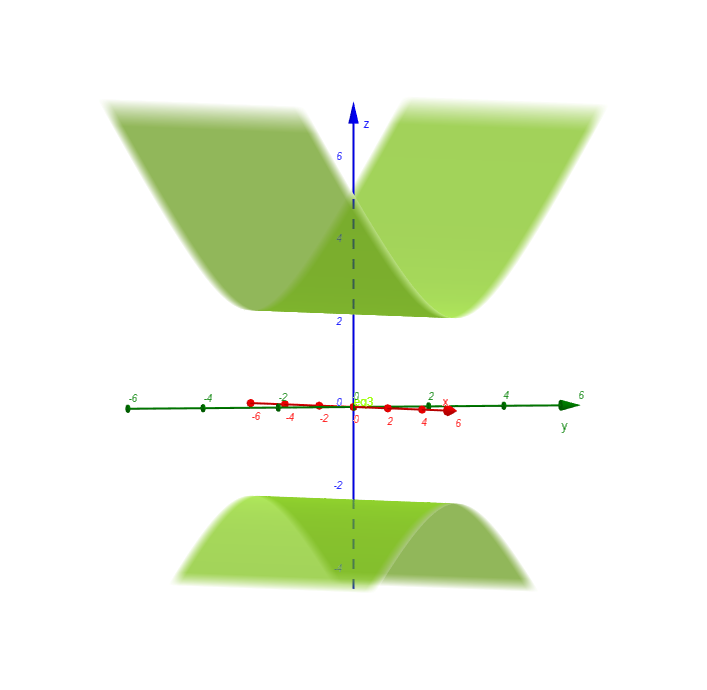
\includegraphics[width=9cm]{img/2e1}
		\caption{Tomaremos la superficie verde claro }
		\label{F1_1}
	\end{subfigure}
	\begin{subfigure}{0.3\textwidth}
		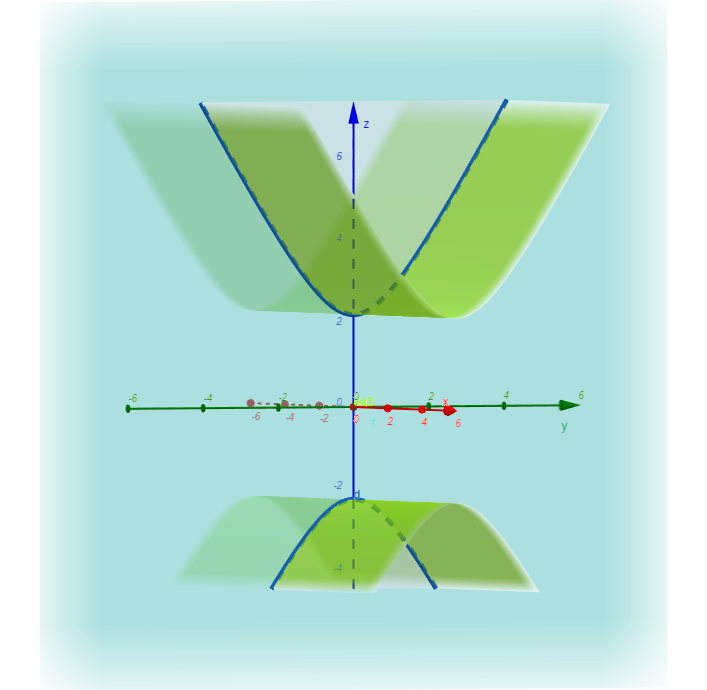
\includegraphics[width=\linewidth]{img/2e2_1}
		\caption{Con $ x = 1 $}
	\end{subfigure}
	\begin{subfigure}{0.3\textwidth}
		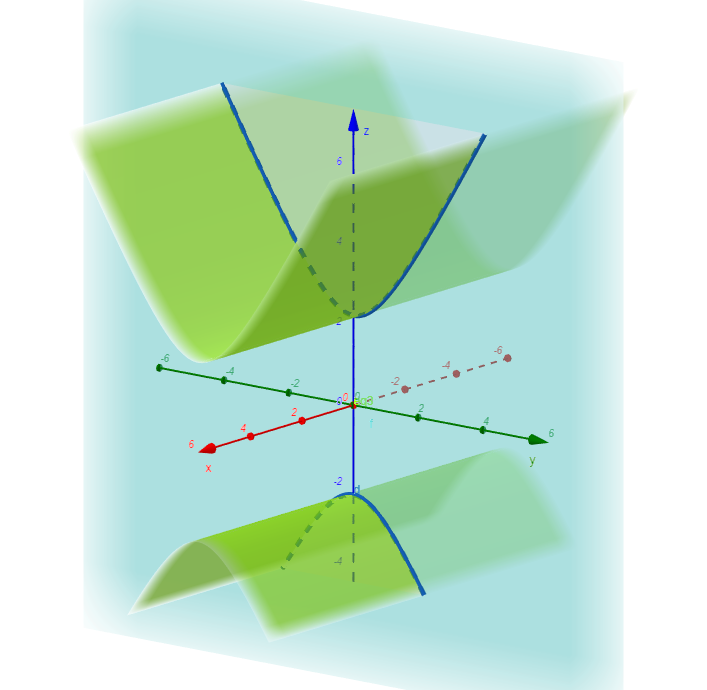
\includegraphics[width=\linewidth]{img/2e2_2}
		\caption{Para $ y = 0 $}
	\end{subfigure}
	\begin{subfigure}{0.3\textwidth}
		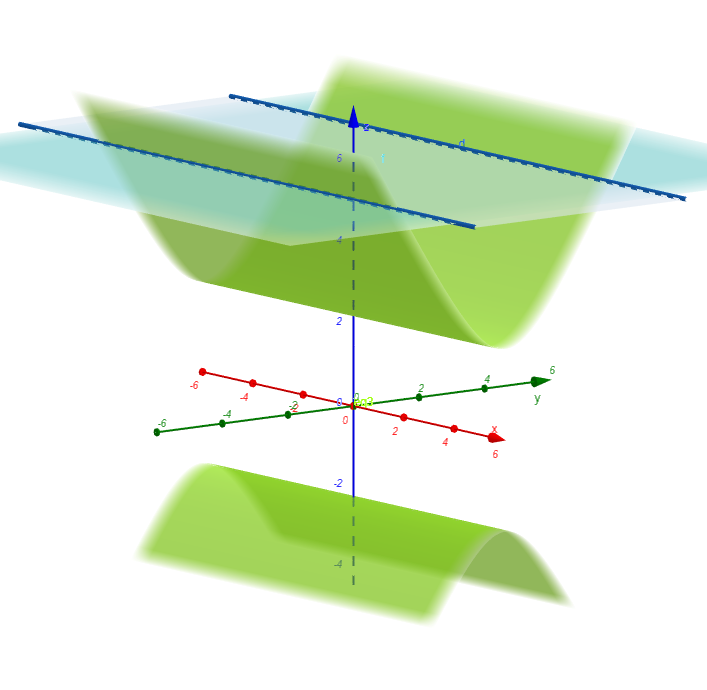
\includegraphics[width=\linewidth]{img/2e2_3}
		\caption{Para $ z = 8 $}
	\end{subfigure}
	\caption{Secciones de la gráfica }
\end{figure}

\end{enumerate}




\end{document}
